% latex2e header
\documentclass[11pt]{article}
\usepackage{latexsym}
\usepackage{fullpage}
\usepackage{fancyhdr}
\usepackage{graphicx}
%\usepackage{pstricks}
%\usepackage{psfig}
%\pagestyle{fancyplain}
\pagestyle{empty}
\topmargin   -0.70in

%\input{lab-fmt.tex}
\input epsf.sty
%\setcounter{laboratory}{2} %one less
\def\half{{\textstyle {1\over2}}}
\def\3half{{\textstyle {3\over2}}}

\setlength{\textheight}{10.5in}


\begin{document}
\thispagestyle{empty}
Professor Fearing ~~~~~~~~~~ EECS 192 Worksheet 1 DC Motor ~~~~~~~~~~~~~ Spring 2015\\

*** For practice, not collected or graded ***

\begin{tabular}{c}
  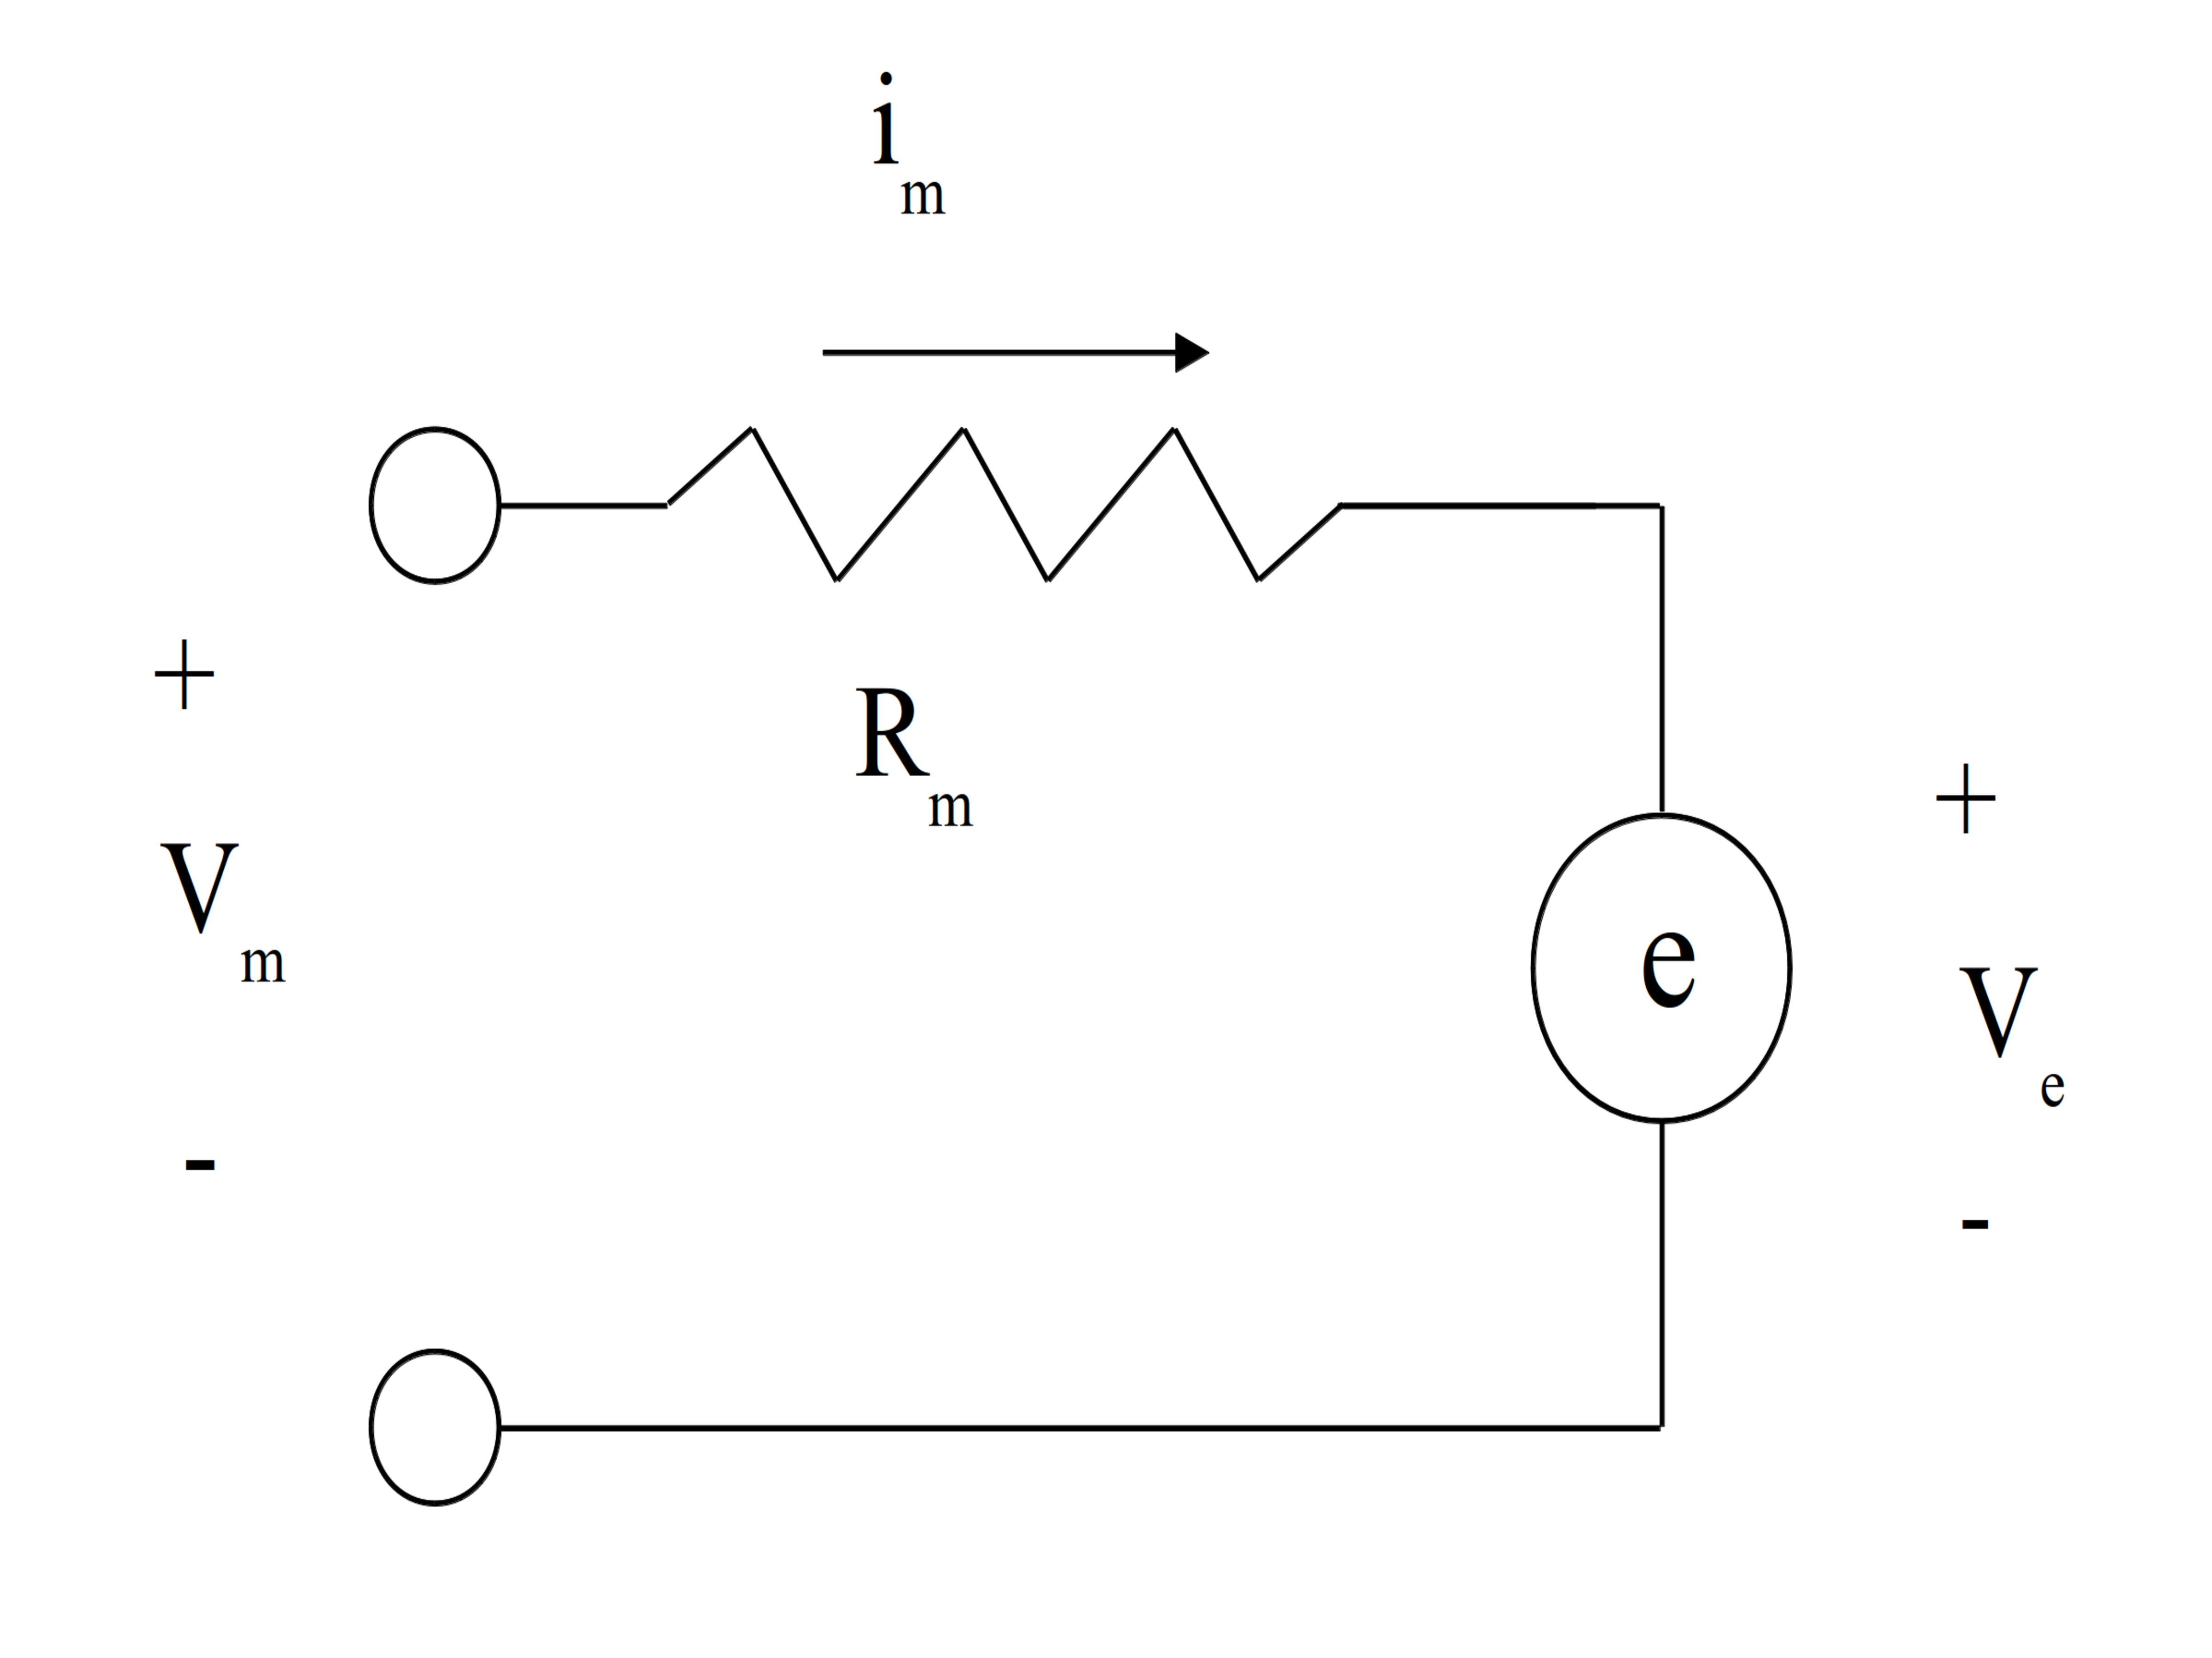
\includegraphics[scale=0.3]{motor-model.png} \\
Fig. 1 Simplified motor model without inductance.\\ 
Given: $R_m = 2 \Omega$, $k_\tau = 0.1 N m^{-1}$, $k_e = 0.01 V- s/rad$\\
\end{tabular}
\vspace{0.1in}

As derived in class, the motor torque depends on motor current:
$ \tau = k_\tau i_m $, 
where $\tau$ has units of $N-m$, and $k_\tau$ is $N-m/amp$.\\

The back emf voltage is proportional to motor velocity:
$ V_e = k_e \dot{\theta}_m $, 
where $\dot{\theta}_m $ is motor velocity in radians/second and thus $k_e$ has units of $ Volt - sec/ rad$.\\


For the physics behind the motor model, see:\\
{\verb http://higheredbcs.wiley.com/legacy/college/nise/0470646128/appendices/appendixI.pdf }

\vspace{0.1in}

{\bf Problems:}\\

1. The unloaded motor is connected to a 6V battery. 
Neglecting friction and other losses, determine $i_m, V_e$, and $\dot{\theta}_m$ in steady state.\\

2. The motor is connected to a 6V battery with negligible internal battery
resistance. The motor shaft is clamped so that $\dot{\theta}_m = 0$.\\
Determine $i_m, V_e$, and $\tau_m$.\\

3. The motor is connected through a gear box to a car tire. The motor 
is turning at 5000 rpm. What is the instantaneous 
open circuit voltage $V_m$?\\

4. The motor is turning at 5000 rpm, and $V_m$ is now short circuited.
What is the initial current $i_m$, and torque $\tau_m$ shortly 
after the short circuit is applied?\\

For the following, consider that
the motor is connected through a gear box to a car tire. The motor is 
initially turning at 5000 rpm, and the car has inertia and friction.\\

5. Consider $V_m$ is short circuited at $t=0$.
Sketch the trend of $i_m, V_e, \dot{\theta}_m$,
and $\tau_m$  until the car comes to a rest.\\

6. Consider now $V_m$ is short circuited for 1 ms at t=0. 
Sketch variables as above for -1 ms $< t <$ 2 ms.\\

7. Consider now $V_m$ is connected to a 6V battery with 
negligible internal resistance at $t = 0$ ms. 
Sketch the trend of $i_m, V_e, \dot{\theta}_m$,
and $\tau_m$  until the car reaches a steady state velocity.\\

8. Consider now $V_m$ is connected to the 6V battery for 1 ms at t=0, and then
$V_m$ is open circuited. 
Sketch variables as above for -1 ms $< t <$ 2 ms.\\


\end{document}
